%------------------------------------------%
%
% Cannabis Data Science
% Saturday Morning Statistics
%
% Date: 4/2/2022
%
%------------------------------------------%
\documentclass[xcolor={dvipsnames}]{beamer}
\hypersetup{pdfpagemode = FullScreen}
\mode<presentation>{
  \usetheme{Boadilla}
  \usecolortheme{orchid}
  \usefonttheme{default}
  \setbeamertemplate{navigation symbols}{}
  \setbeamertemplate{caption}[numbered]
}
\setbeamersize{
  text margin left = 0.5in,
  text margin right = 0.5in
}

%------------------------------------------%
% Title
%------------------------------------------%
\author{Cannabis Data Science}
\title[\textbf{Saturday Morning Statistics \#18}]{}
\institute[]{\Large Saturday Morning Statistics \#18}
\date{April \nth{2}, 2022}

%------------------------------------------%
% Packages
%------------------------------------------%
\usepackage[english]{babel}
\usepackage[utf8x]{inputenc}
\usepackage{tikz}
\usepackage{xparse}

%------------------------------------------%
% Colors
%------------------------------------------%
\definecolor{Green}{RGB}{34, 153, 84}
\definecolor{LightGreen}{RGB}{218, 247, 166}
\definecolor{DarkGreen}{RGB}{2, 48, 32}
\definecolor{Orange}{RGB}{255, 87, 51}
\definecolor{DarkOrange}{RGB}{199, 0, 57}
\definecolor{Yellow}{RGB}{255, 195, 0}

%------------------------------------------%
% Theme
%------------------------------------------%
\setbeamercolor*{palette primary}{bg=LightGreen, fg=DarkGreen}
\setbeamercolor*{palette secondary}{bg=LightGreen, fg=DarkGreen}
\setbeamercolor*{palette tertiary}{bg=LightGreen, fg=DarkGreen}

%------------------------------------------%
% Packages
%------------------------------------------%
\usepackage{amsmath}
\renewcommand*\footnoterule{} % No separating line on footnote.
\usepackage{mathtools} % For annotating equations.
\usepackage{hhline} % for double bars.
\usepackage[super]{nth} % For formatting 1st, 2nd, 3rd, etc.
\usepackage{graphicx, caption, subcaption}
\usepackage{setspace}
%\usepackage{enumitem}

%------------------------------------------%
% Commands
%------------------------------------------%

% Top space.
\newcommand\T{\rule{0pt}{2.5ex}}

% Bottom space.
\newcommand\B{\rule[-1.25ex]{0pt}{0pt}}

% Blocks.
\newenvironment<>{Block}[2][.9\textwidth]
  {\setlength{\textwidth}{#1}
  \begin{actionenv}#3
    \def\insertblocktitle{#2}\par
    \usebeamertemplate{block begin}}
  {\par\usebeamertemplate{block end}
  \end{actionenv}}

% Balls.
\defbeamertemplate{enumerate item}{largeball}
{\begin{pgfpicture}{-1ex}{-0.65ex}{1.5ex}{1.5ex}
\usebeamercolor[fg]{item projected}
{\pgftransformscale{2.5}\pgftext{\Large\pgfuseshading{bigsphere}}}
{\pgftransformshift{\pgfpoint{0pt}{0.5pt}}
\pgftext{\usebeamerfont*{item projected}\small\insertenumlabel}}
\end{pgfpicture}}

% Fancy arrows.
\NewDocumentCommand\UpArrow{O{2.0ex} O{black}}{%
   \mathrel{\tikz[baseline] \draw [->, line width=0.5pt, #2] (0,0) -- ++(0,#1);}} % Fancy up-arrow.
\NewDocumentCommand\DownArrow{O{2.0ex} O{black}}{%
   \mathrel{\tikz[baseline] \draw [<-, line width=0.5pt, #2] (0,0) -- ++(0,#1);}} % Fancy down-arrow.

% Equations with numbers on the left.
\makeatletter
\newcommand{\LeftEqNo}{\let\veqno\@@leqno}
\makeatother

%------------------------------------------%
%
% Presentation
%
%------------------------------------------%
\begin{document}

%------------------------------------------%
% Title Page
%------------------------------------------%
\begin{frame}{}
  
\includegraphics[scale=0.33]{images/logo.pdf}
  \vspace*{-2\baselineskip}
  \titlepage
\end{frame}


%------------------------------------------%
% Question and Hypothesis
%------------------------------------------%
\section{Question and Hypothesis}
\begin{frame}{Question and Hypothesis}

% Question of the day
\begin{center}
\begin{minipage}{.9\linewidth}
\begin{Block}{Question of the day.}

\vspace{.5\baselineskip}
\begin{itemize}

\item What can producers do to minimize their risk of quality control testing?

\end{itemize}

\vspace{.5\baselineskip}

\end{Block}
\end{minipage}
\end{center}

\vspace{.25\baselineskip}
\begin{center}
\begin{minipage}{0.6\textwidth}
\begin{figure}
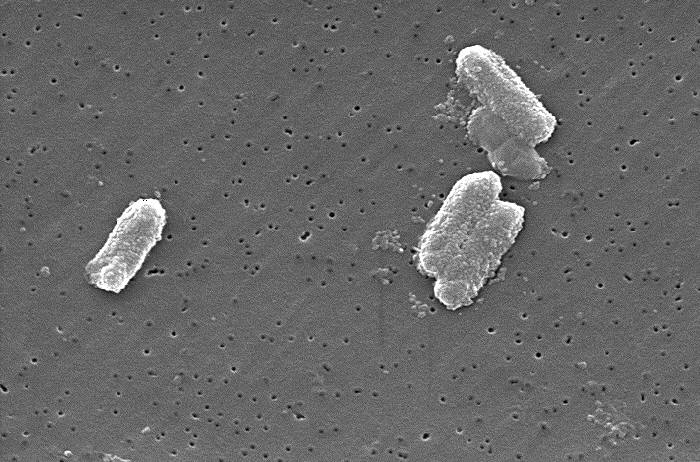
\includegraphics[width=2in]{images/entero.jpg}
\caption*{
\scriptsize {\itshape Citrobacter freundii}, one member of the family {\bfseries Enterobacteriaceae} -- bile tolerant gram negative bacteria (BTGN).
}
\end{figure}
\end{minipage}
\end{center}


\end{frame}


%------------------------------------------%
% Methodology: Probit Models
%------------------------------------------%

\begin{frame}{Methodology: Probit Models}

Given a latent variable representation of the {\bfseries probit model}:

\begin{align*}
z_i &= x_i\beta + \epsilon _i, \hspace{4ex} \epsilon _i \stackrel{iid}{\sim} \mathcal{N}(0, 1), \\
\\[-0.5\baselineskip]
y_i &=
  \begin{cases}
    1 \text{ if } z_i > 0\\
    0 \text{ if } z_i \leq 0
  \end{cases}
\end{align*}

\vspace{0.5\baselineskip}
You can estimate the parameters using the {\bfseries likelihood function}

$$
L(\beta) = \prod_{i=1}^n\Phi(x_i\beta)^{y_i}[1 - \Phi(x_i\beta)]^{1-y_i}.
$$

\end{frame}



%------------------------------------------%
% Tobit Models
%------------------------------------------%

\begin{frame}{Methodology: Tobit Models}

{\bfseries Tobit models} incorporate the \underline{unequal sampling probability} for each observation depending on whether the latent dependent variable fell above or below the determined \underline{threshold}.

\vspace{1\baselineskip}
\begin{itemize}

\item Censored from below at $y_{L}$ when the latent variable $y_{j}^{*}\leq y_{L}$

$$
I(y) = \begin{cases}
0 \text{ if } y \leq y_L,\\
1 \text{ if } y > y_L
\end{cases}
$$

\vspace{0.5\baselineskip}
\item Censored from above at $y_{U}$ when the latent variable $y_{j}^{*}\geq y_{U}$

$$
I(y) = \begin{cases}
0 \text{ if } y \geq y_U,\\
1 \text{ if } y < y_U
\end{cases}
$$

\end{itemize}

%------------------------------------------%
% Estimating Tobit Models
%------------------------------------------%

\end{frame}


\begin{frame}{Estimating Tobit Models}


A {\bfseries Tobit model} modifies the \underline{likelihood function} to reflect the \underline{unequal sampling probability}

$$
\mathcal{L}(\beta,\sigma) = \prod_{j=1}^N\left(\frac{1}{\sigma}\phi\left(\frac{y_j - X_j\beta}{\sigma}\right)\right)^{I(y_j)}\left(1 - \Phi\left(\frac{X_j\beta - y_L}{\sigma}\right)\right)^{1-I(y_j)},
$$

\vspace{0.5\baselineskip}
where $\phi$ is the {\bfseries standard normal PDF} and $\Phi$ is the {\bfseries standard normal CDF}.

\end{frame}

%------------------------------------------%
% Interpreting Tobit Models
%------------------------------------------%

\begin{frame}{Interpreting Tobit Models}

\begin{itemize}

\item Tobit models allow for {\bfseries consistent} parameter estimation. If $y_i$ is regressed on $x_i$ alone, then the parameter $\beta$ is {\bfseries inconsistent} ($\hat{\beta}$ does not converge in probability to $\beta$).

\vspace{1\baselineskip}

\item The parameter $\beta$ is interpreted as

\vspace{1\baselineskip}
\begin{enumerate}

\item The change in $y_{i}$ of those above the limit, weighted by the probability of being above the limit;

\vspace{1\baselineskip}

\item The change in the probability of being above the limit, weighted by the expected value of $y_{i}$ if above the limit.

\end{enumerate}

\end{itemize}

\end{frame}

%------------------------------------------%
% Types of Tobit Models
%------------------------------------------%

\begin{frame}{Types of Tobit Models}

{\bfseries Type 1} Tobit models censor at a value different from zero

$$
y_i = \begin{cases}

y_i^* \text{ if } y_L < y_i^* < y_U, \\
y_L \text{ if } y_i^* \leq Y_L,\\
y_U \text{ if } y_i^* \geq y_U.
\end{cases}
$$

\vspace{1\baselineskip}
{\bfseries Type 2} Tobit models ({\bfseries Heckman selection models}), introduce a second latent variable to allow the process of participation (selection) and the outcome of interest to be independent

$$
y_{2i} = \begin{cases}
y_{2i}^* \text{ if } y_{1i}^* > 0,\\
0 \text{ if } y_{1i}^* \leq 0.
\end{cases}
$$

\vspace{1\baselineskip}
{\bfseries Type 3}, {\bfseries Type 4}, {\bfseries Type 5} Tobit models introduce additional cases for additional latent variables.

\end{frame}

%------------------------------------------%
% Takeaway
%------------------------------------------%
\section{Takeaway}
\begin{frame}{}

\begin{center}
\begin{minipage}{3.85in}

% Thank you.
\begin{center}

\includegraphics[width=.25in]{images/prayer.png} {\Large \textbf{Thank you for coming.}}\\
\end{center}
\vspace*{0.5\baselineskip}

% Re-cap the lesson of the day.
\begin{center}
\begin{minipage}{\linewidth}
\begin{Block}{Insight of the Day}

\vspace{0.5\baselineskip}

\begin{itemize}

\item Asking the right question is of utmost importance.

\vspace{0.5\baselineskip}

\end{itemize}

\end{Block}
\end{minipage}
\end{center}

\vspace*{2\baselineskip}

\end{minipage}
\end{center}

\end{frame}


%------------------------------------------%
% Fin.
%------------------------------------------%
\end{document}
